% ---------
% Preamble.
% ---------

% Document type.
\documentclass{article}

% Import custom style.
\usepackage{../.preamble/tikz_diagrams_template}

% Color theme (black, red, blue, green, orange, purple, gold).
\colortheme{blue}

% ---------
% Document.
% ---------

\begin{document}

    % -----------------
    % TikZ environment.
    % -----------------

    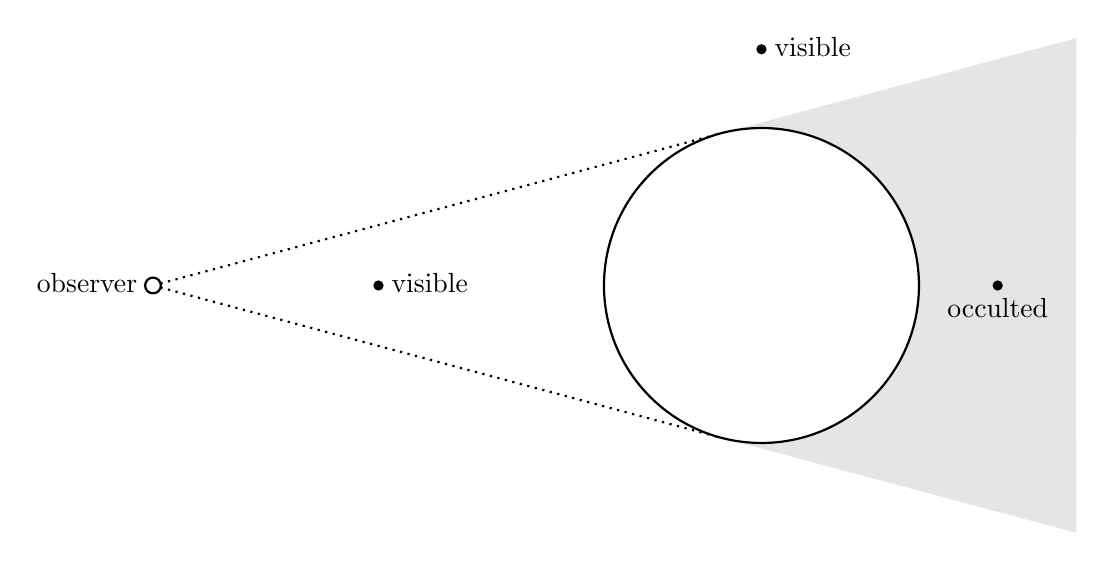
\begin{tikzpicture}

        % -----------
        % Parameters.
        % -----------
        
        % Constants.
        \pgfmathsetmacro{\radiusOcc}{2}         % Occulting body radius.
        \pgfmathsetmacro{\thetaAngle}{15}       % Angle from observer to incidence point [deg].
        \pgfmathsetmacro{\radiusObserver}{0.1}  % Observer radius.
        \pgfmathsetmacro{\radiusTarget}{0.05}   % Target radius.

        % Derived parameters.
        \pgfmathsetmacro{\xObserver}{-\radiusOcc/sin(\thetaAngle)}                      % x-position of observer.
        \pgfmathsetmacro{\thetaAngleComp}{90-\thetaAngle}                               % Complement of theta [deg].
        \pgfmathsetmacro{\xInc}{-\radiusOcc*cos(\thetaAngleComp)}                       % x-position of incidence points.
        \pgfmathsetmacro{\yIncUpper}{\radiusOcc*sin(\thetaAngleComp)}                   % y-position of upper incidence point.
        \pgfmathsetmacro{\yIncLower}{-\yIncUpper}                                       % y-position of lower incidence point.
        \pgfmathsetmacro{\xShadowEnd}{2*\radiusOcc}                                     % x-position of shadow end.
        \pgfmathsetmacro{\yShadowEndUpper}{(\xShadowEnd-\xObserver)*tan(\thetaAngle)}   % y-position of upper shadow end.
        \pgfmathsetmacro{\yShadowEndLower}{-\yShadowEndUpper}                           % y-position of lower shadow end.
        \pgfmathsetmacro{\xTargetVisibleOne}{0.5*(\xObserver-\radiusOcc)}               % x-position of 1st visible target.
        \pgfmathsetmacro{\yTargetVisibleTwo}{1.5*\radiusOcc}                            % y-position of 2nd visible target.
        \pgfmathsetmacro{\xTargetOcculted}{1.5*\radiusOcc}                              % x-position of occulted target.

        % --------
        % Drawing.
        % --------

        % Lines to incidence points.
        \draw[dotted,thick](\xObserver,0)--(\xInc,\yIncUpper);
        \draw[dotted,thick](\xObserver,0)--(\xInc,\yIncLower);

        % Cylindrical portion of shadow.
        \fill[gray!20](\xInc,\yIncLower)rectangle(\xShadowEnd,\yIncUpper);

        % Upper slanted portion of shadow.
        \fill[gray!20](\xInc,\yIncUpper)--(\xShadowEnd,\yIncUpper)--(\xShadowEnd,\yShadowEndUpper)--cycle;

        % Lower slanted portion of shadow.
        \fill[gray!20](\xInc,\yIncLower)--(\xShadowEnd,\yIncLower)--(\xShadowEnd,\yShadowEndLower)--cycle;
        
        % Occulting body.
        \draw[thick,fill=white](0,0)circle(\radiusOcc);
        
        % Observer.
        \draw[thick,fill=white](\xObserver,0)circle(\radiusObserver)node[left,xshift=-2,yshift=1]{observer};

        % Visible target #1.
        \draw[thick,fill=black](\xTargetVisibleOne,0)circle(\radiusTarget)node[right,xshift=1,yshift=1]{visible};

        % Visible target #2.
        \draw[thick,fill=black](0,\yTargetVisibleTwo)circle(\radiusTarget)node[right,xshift=1,yshift=1]{visible};

        % Occulted target.
        \draw[thick,fill=black](\xTargetOcculted,0)circle(\radiusTarget)node[below,yshift=-1]{occulted};

    \end{tikzpicture}

\end{document}
